\NeedsTeXFormat{LaTeX2e}[1995/12/01]
\documentclass[10pt]{bmc_article}    

\usepackage{cite} % Make references as [1-4], not [1,2,3,4]
\usepackage{url}  % Formatting web addresses  
\usepackage{ifthen}  % Conditional 
\usepackage{multicol}   %Columns
\usepackage[utf8]{inputenc} %unicode support
%\usepackage[latin1]{inputenc} %UNIX support if unicode package fails
\urlstyle{rm}
\usepackage[pdftex]{graphicx}
 
%\def\includegraphic{}
%\def\includegraphics{}

\setlength{\topmargin}{0.0cm}
\setlength{\textheight}{21.5cm}
\setlength{\oddsidemargin}{0cm} 
\setlength{\textwidth}{16.5cm}
\setlength{\columnsep}{0.6cm}

\newboolean{publ}

\newenvironment{bmcformat}{\begin{raggedright}\baselineskip20pt\sloppy\setboolean{publ}{false}}{\end{raggedright}\baselineskip20pt\sloppy}

%Publication style settings
%\newenvironment{bmcformat}{\fussy\setboolean{publ}{true}}{\fussy}

% Begin ...
\begin{document}
\begin{bmcformat}

\title{Resource Description Framework Technologies in Chemistry}
 
\author{Egon L Willighagen\correspondingauthor$^{1}$%
       \email{Egon L Willighagen\correspondingauthor - egon.willighagen@ki.se}%
       and 
         Martin P Br\"andle$^2$%
         \email{Martin P Br\"andle - braendle@chem.ethz.ch}%
      }

\address{%
    \iid(1)Division of Molecular Toxicology, Institute of Environmental Medicine, Karolinska Institutet, SE-17177 Stockholm, Sweden\\
    \iid(2)Chemistry Biology Pharmacy Information Center, ETH Z\"urich, Wolfgang-Pauli-Str. 10, 8093 Z\"urich, Switzerland
}%

\maketitle


%\begin{abstract}
%        \paragraph*{Background:} Text for this section of the abstract. 
%        \paragraph*{Results:} Text for this section of the abstract \ldots
%        \paragraph*{Conclusions:} Text for this section of the abstract \ldots
%\end{abstract}

% I don't think an abstract is required for an Editorial/mb

The Resource Description Framework (RDF) is providing the life sciences with new standards
around data and knowledge management. The uptake in the life sciences is
significantly higher than the uptake of the eXtensible Markup Language (XML)
and even relational databases, as was recently shown by Splendiani et
al.~\cite{Splendiani2011} Chemistry is adopting these methods too.
For example, Murray-Rust and coworkers used RDF already in 2004 to distribute
news items where chemical structures were embedded using RDF Site Summary 1.0.~\cite{MurrayRust2004}
Frey implemented a system which would now be referred to an
electronic lab notebook (ELN).~\cite{Frey2004} The use of the SPARQL
query language goes back to 2007 where it was used in a system to annotate
crystal structures.~\cite{Hunter2007}

The American Chemical Society (ACS) Division of Chemical Information (CINF)
invited scientists from around the world to present their use of RDF
technologies in chemistry on 22nd-23rd August 2010
at the 240th ACS National Meeting in Boston, USA. During three half-day
sessions, the speakers demonstrated a mix of smaller and larger initiatives
where RDF and related technologies are used in cheminformatics and
bioinformatics as Open Standards for data exchange, common languages
(ontologies), and problem solving. The fifteen presentations were grouped in the themes computation,
ontologies, and chemical applications. Figures~1 to~3 display the most important
keywords reflecting the abstracts of the talks in each session as word
clouds~\cite{WORDLE}.

The goal of the meeting was to make more chemists aware of what the RDF Open
Standard has to offer to chemistry. We are delighted to continue this effort
with this thematic issue, for which the speakers (and others) were invited
to present their work in more detail to a wider chemistry community. The choice
of an Open Access journal follows this goal. At this place, we would like to thank Pfizer, Inc., 
who had partially funded the article processing charges for this Thematic Series.
Pfizer, Inc. has had no input into the content of the publication or the articles themselves.
All articles in the series were independently prepared by the authors and
were subjected to the journal's standard peer review process.

In the remainder of this editorial, we will briefly outline the various RDF
technologies and how they have been used in chemistry so far.

\section{Concepts}

The core RDF specification was introduced by the World Wide Web Consortium (W3C)
in 1999~\cite{Lassila1999} and defines the foundation of the RDF technologies. It has
evolved into a set of six recommendations by W3C published in 2004
(See Table~1). 
RDF specifies a very simple data structure linking a subject to an object or a
value (literal) using a predicate. Cheminformaticians will recognize this data
structure as an edge from graph theory. This structure allows us to represent
facts like ``vanillin dissolves in methyl alcohol''~\cite{ONS2010}. RDF uses Uniform
Resource Identifiers (URIs) to identify things. Therefore, the RDF equivalent of
the solution statement could be like this so-called triple:

\vspace{0.3cm}
\begin{small}
http://dbpedia.org/resource/Vanillin http://example.com/dissolvesIn http://dbpedia.org/resource/Methanol .
\end{small}
\vspace{0.3cm}

Since URIs may be used to reference resources on any server worldwide,
RDF triples allow to span a global graph data structure. 
This is not surprising, since RDF is the core technology behind the
proposed Semantic Web~\cite{BER2001}. In fact, the Web
nature is clear here, as one can follow both the URIs for vanillin and methanol to
obtain further information on those two chemicals. These molecules' URIs are said to be
dereferencable, allowing agents to spider the Web for information following
the hyperlinks, quite like how you follow hyperlinks on websites. Hence, the term Semantic Web.

Recent projects such as Bio2RDF~\cite{BEL2008}, Chem2Bio2RDF~\cite{CHE2010},
and OpenTox~\cite{Hardy2010} have brought genomic, pharmaceutical and
chemical knowledge to the Semantic Web by expressing it in RDF.
These three projects aim at making databases with chemical knowledge
available from a central access point, interlinking the individual
data sets. Smaller data sets are also becoming available as RDF, such as
the Open Notebook Science Solubility data~\cite{citeulike:5441072}. 

\section{Formats}

The actual use of RDF depends on various further standards. For example, standards were required
that describe how RDF statements are exchanged. Several standards
serve this purpose: RDF/XML is an XML-based serialization~\cite{Beckett2004}, while
simpler formats exist with N-Triples~\cite{Beckett2004b} and Notation3.~\cite{BernersLee2006} For integration with
current web practices, RDFa has been defined to allow RDF triples to be embedded
in HTML pages.~\cite{RDFA2008} Additionally, a proposal has been written that
describe how RDF can be serialized as Javascript Object Notation (JSON)~\cite{Alexander2008}, and
while this is not a formal specification yet,
a new RDF working group will formalize this into a new standard.~\cite{Herman2010} Several
of these serialization standards are used in the papers in this Series.

Using these serializations, RDF can be downloaded directly from pure RDF
documents (RDF/XML, Notation3), or extracted from RDFa-based web pages using
online RDF extraction web services, like http://www.w3.org/2007/08/pyRdfa/.
These approaches make it simple to aggregate chemical data from web pages.

\section{Querying the World Wide Web}

The most promising technology in the RDF family is the
SPARQL Protocol and RDF Query Language (SPARQL)~\cite{PrudHommeaux2008}, which has been
applied by Chen et al. in three chemogenomics use cases.~\cite{CHE2010}
One of the use cases shows how SPARQL queries are used to find compounds 
that are active in bioassay for genes related to proteins
to which the chemical dexamethasone binds, using information
from PubChem, Uniprot, and DrugBank, all made available as RDF in the Chem2Bio2RDF
database. The other use cases in this paper use the same approach
by aggregating data sources before querying them. As such, it is similar to
querying data stored in a relational database.
However, an important difference between SPARQL and SQL query engines is
the underlying data they act on: a graph of triples for RDF data, and
rectangular tables in relational databases.
This difference implies that RDF resources must have at least some
common elements,  whereas a relational DBMS assumes an identical data
structure for all records of a table."

For example, Jankowski used a public
SPARQL service to extract boiling points of a series of alkanes from an XHTML
webpage with the data made machine readable with RDFa, and visualized that using
Javascript in another web page dynamically~\cite{Jankowski2010} (see
Figure~4). A second important difference is that SPARQL queries can be
\textit{federated}.~\cite{Prudhommeaux2007Custom}
Federated SPARQL allows one to query various RDF providers in one query. This has
been used recently in the Receptor Explorer tool to help translational research
by connecting basic neuroscience research with clinical trials~\cite{Cheung2009}.
Being able to query resources in this manner, brings us a step closer to
systems biology approaches.

\section{Ontologies}

With RDF we have a data structure to link resources and provide details about
those resources, and SPARQL provides us with the tools to query and aggregate that data.
The next standard we will discuss now is the Web Ontology
Language (OWL) which brought the RDF technology to the ontology community~\cite{GUN2004}.
Ontologies are most certainly not new to chemistry~\cite{Gordon1988} nor biology or life sciences,
but the OWL standard makes it much easier to use ontologies, partly because
they are formulated in RDF themselves. Ontologies, like
controlled vocabularies and thesauri, describe what things mean, by linking
terms to a human-readable definition. As such, ontologies are used for sharing
knowledge in a common language, as well as to organize that knowledge.
While linking resources is not new either, expressing the content of resources
in explicit terms allows humans and software to reason formally on the content and to find possible sources of error.
For example, Konyk et al. have used OWL to link PubChem,
DrugBank, and DBPedia, noting that it offers new ways to
discover knowledge~\cite{Konyk2008}.

%mb changed phrase "While ..."

There are currently not many ontologies in chemistry, but many OBO Foundry-based
ontologies can be reused using an OBO to OWL mapping.~\cite{Moreira2007} This makes
available chemical ontologies like the CO ontology~\cite{Feldman2005},
the ontology of Chemical Entities of Biological Interest (ChEBI)~\cite{Degtyarenko2008,Hull2008},
and the Cheminformatics Ontology (\url{http://code.google.com/p/semanticchemistry/}),
but also other ontologies in the life sciences, such as the Gene Ontology.~\cite{Aranguren2007}
This way, OWL provides a universal standard to link data sources in life
sciences, transcending traditionally boundaries between the various domains.

The current state is that different RDF resources are using different ontologies.
This does not necessarily have to be a problem, because the ontologies can be
explicitly mapped to each other. This way, equivalent terms from two ontologies
can be formally defined as equivalent, using the OWL predicates owl:equivalentClass
and owl:equivalentProperty for classes, and owl:sameAs for instances.
Making the equivalence explicit this way helps to illustrate the provenance of data integration efforts. 

%mb Improved "Making the equivalence ..."

\section{Discussion}

This Thematic Series shows the current state of the use of RDF in
chemistry, as presented at the ACS RDF 2010 meeting in Boston, and provides an
insight into the progress of these methods. Much of the research is currently explorative,
rather than formative, though standards are being proposed.
It may very well turn out that some aspects of chemistry will never be expressed
in RDF, and some computation will be done without ontology-based reasoning. It is important
to realize here where RDF is positioned, namely for linking resources.

However, the use of RDF for already well-defined data structures in chemistry
is not obvious. Data types like connection tables and various matrices are possible, 
but the use of URIs makes such structures needlessly verbose.
Moreover, there is no need to format already well-formalized data structures into
RDF, such as the various uses of matrices in computational chemistry as
RDF triples.
In fact, several papers in this series outline how to
combine knowledge expressed with RDF with computational services.
This shows that RDF is not an isolated framework, but one that can be
integrated into existing cheminformatics workflows.

What RDF does not solve, are the following issues that remain in
cheminformatics. RDF is about knowledge representation, and while
ontologies take care of meaning and provide requirements to verify formal data consistency, 
it does not enfore any data quality, data structure, or data availability. 
This is, in fact, similar to other
ways of providing data. For example, a data set with boiling points
may or may not include information about experimental error.
Metabolomics data may name the molecules for which concentration
profiles have been measure, or the original accurate masses from
which the identity was deduced.

%mb improved "RDF is about knowledge representation, ..."

It must be clear, therefore, that the RDF technologies are not the solution
to everything. Their use does not garantee an impressive scientific
scenario. Instead, it can help simplify data analysis and particularly
data integration, making it easier to handle large volumes of
data accurately, or at least, with a explicitly defined accuracy.

As such, the use of explicit, semantic formats can be considered
a gold standard of scientific practise. It's about adding as much detail
to your lab notebook as you need. But, it does not inhibit you
from writing non-sense in your notebook.

\section{Outlook}

The future of the use of RDF technologies as open standards in chemistry looks
bright, and fills the needs in chemistry for semantically linking
chemical data to other data sources. RDF technologies provide a
domain-independent way for representing knowledge and its open
nature assures many alternative approaches for making data available
as RDF.
This Thematic Series shows a few novel and creative applications of
these RDF technologies, and we hope they may serve as seminal work
in cheminformatics for future years.

\ifthenelse{\boolean{publ}}{\begin{multicols}{2}}{}


%{\ifthenelse{\boolean{publ}}{\footnotesize}{\small}
% \bibliographystyle{bmc_article}  % Style BST file
%  \bibliography{editorial} }     % Bibliography file (usually '*.bib' ) 

%% BioMed_Central_Bib_Style_v1.01

\begin{thebibliography}{10}
\providecommand{\url}[1]{[#1]}
\providecommand{\urlprefix}{}

\bibitem{Splendiani2011}
Splendiani A, Burger A, Paschke A, Romano P, Marshall M: \textbf{Biomedical
  semantics in the Semantic Web}. \emph{J Biomed Semantics} 2011,
  \textbf{2}(Suppl 1):S1.

\bibitem{MurrayRust2004}
Murray-Rust P, Rzepa HS, Williamson MJ, Willighagen EL: \textbf{Chemical
  markup, {XML}, and the World Wide Web. 5. Applications of chemical metadata
  in {RSS} aggregators.} \emph{J Chem Inf Comput Sci} 2004,
  \textbf{44}(2):462--469.

\bibitem{Frey2004}
Frey JG: \textbf{Dark Lab or Smart Lab: The Challenges for 21st Century
  Laboratory Software}. \emph{Org Process Res Dev} 2004,
  \textbf{8}(6):1024--1035.

\bibitem{Hunter2007}
Hunter J, Henderson M, Khan I: \textbf{Collaborative Annotation of {3D}
  Crystallographic Models}. \emph{J Chem Inf Model} 2007,
  \textbf{47}(6):2475--2484.

\bibitem{WORDLE}
\textbf{Wordle}. \emph{http://www.wordle.net/}.

\bibitem{Lassila1999}
Lassila O, Swick RR: \textbf{Resource Description {Framework(RDF}) Model and
  Syntax Specification}.
  \emph{http://www.w3.org/TR/1999/REC-rdf-syntax-19990222} 1999.

\bibitem{ONS2010}
Bradley JC, Friesen B, Mancinelli J, Bohinski T, Mirza K, Bulger D, Moritz M,
  Federici M, Rein D, Tchakounte C, Bradley JC, Truong H, Neylon C, Guha R,
  Williams A, Hooker B, Hale J, Lang A, Bradley JC, Neylon C, Guha R, Williams
  AJ, Hooker B, Lang ASID, Friesen B, Bohinski T, Bulger D, Federici M, Hale J,
  Mancinelli J, Mirza KB, Moritz MJ, Rein D, Tchakounte C, Truong HT:
  \textbf{Open Notebook Science Challenge: Solubilities of Organic Compounds in
  Organic Solvents}. \emph{Available from Nature Precedings
  $<$http://dx.doi.org/10.1038/npre.2010.4243.2$>$} 2010.

\bibitem{BER2001}
Berners-Lee T, Hendler J, Lassila O: \textbf{The Semantic Web}. \emph{Sci Am}
  2001, \textbf{284}(5):34--43.

\bibitem{BEL2008}
Belleau F, Nolin M, Tourigny N, Rigault P, Morissette J: \textbf{{Bio2RDF}:
  Towards a mashup to build bioinformatics knowledge systems}. \emph{J Biomed
  Inf} 2008, \textbf{41}(5):706--716.

\bibitem{CHE2010}
Chen B, Dong X, Jiao D, Wang H, Zhu Q, Ding Y, Wild D: \textbf{{Chem2Bio2RDF}:
  a semantic framework for linking and data mining chemogenomic and systems
  chemical biology data}. \emph{BMC Bioinf} 2010, \textbf{11}:255.

\bibitem{Hardy2010}
Hardy B, Douglas N, Helma C, Rautenberg M, Jeliazkova N, Jeliazkov V, Nikolova
  I, Benigni R, Tcheremenskaia O, Kramer S, Girschick T, Buchwald F, Wicker J,
  Karwath A, Gutlein M, Maunz A, Sarimveis H, Melagraki G, Afantitis A,
  Sopasakis P, Gallagher D, Poroikov V, Filimonov D, Zakharov A, Lagunin A,
  Gloriozova T, Novikov S, Skvortsova N, Druzhilovsky D, Chawla S, Ghosh I, Ray
  S, Patel H, Escher S: \textbf{Collaborative development of predictive
  toxicology applications}. \emph{J Cheminf} 2010, \textbf{2}:7.

\bibitem{citeulike:5441072}
Bradley JC, Guha R, Lang A, Lindenbaum P, Neylon C, Williams A, Willighagen EL:
  \emph{Beautifying Data in the Real World}, Sebastopol, US: O'Reilly Media,
  Inc. 2009 chap.~16.

\bibitem{Beckett2004}
Beckett D: \textbf{{RDF}/XML Syntax Specification (Revised)}.
  \emph{http://www.w3.org/TR/2004/REC-rdf-syntax-grammar-20040210/} 2004.

\bibitem{Beckett2004b}
Beckett D, Grant J: \textbf{{RDF} Test Cases}.
  \emph{http://www.w3.org/TR/2004/REC-rdf-testcases-20040210/} 2004.

\bibitem{BernersLee2006}
Berners-Lee T: \textbf{Notation 3 - An readable language for data on the Web}.
  \emph{http://www.w3.org/DesignIssues/Notation3.html} 2006.

\bibitem{RDFA2008}
Adida B, Birbeck M, McCarron S, Pemberton S: \textbf{{RDFa} in {XHTML}: Syntax
  and Processing}. \emph{http://www.w3.org/TR/2008/REC-rdfa-syntax-20081014/}.
  W3C 2008.

\bibitem{Alexander2008}
Alexander K: \textbf{{RDF} in {JSON}}. In \emph{Proceedings of the 4th Workshop
  on Scripting for the Semantic Web, Tenerife, Spain, June 02, 2008},
  \emph{Volume 368 of \emph{CEUR Workshop Proceedings}} 2008.

\bibitem{Herman2010}
Herman I: \textbf{New {RDF} Working Group, {RDF}/{JSON}, {RDF} {API}…}.
  \emph{http://www.w3.org/QA/2010/12/new\_rdf\_working\_group\_rdfjson.html}
  2010.

\bibitem{PrudHommeaux2008}
Prud'hommeaux E, Seaborne A: \textbf{{SPARQL} Query Language for {RDF}}.
  \emph{http://www.w3.org/TR/2008/REC-rdf-sparql-query-20080115/} 2008.

\bibitem{Jankowski2010}
Jankowski O: \textbf{{SPARQL} to Chart}.
  \emph{http://www.pharmash.com/posts/2010-09-27-sparql-to-chart.html} 2010.

\bibitem{Prudhommeaux2007Custom}
Prud'hommeaux E: \textbf{Federated {SPARQL}}.
  \emph{http://www.w3.org/2007/05/SPARQLfed/} 2007.

\bibitem{Cheung2009}
Cheung KH, Frost HR, Marshall MS, Prud'hommeaux E, Samwald M, Zhao J, Paschke
  A: \textbf{A journey to Semantic Web query federation in the life sciences}.
  \emph{BMC Bioinf} 2009, \textbf{10}(Suppl 10):S10.

\bibitem{GUN2004}
McGuinness DL, Van~Harmelen F: \textbf{{OWL} Web Ontology Language Overview}.
  \emph{http://www.w3.org/TR/2004/REC-owl-features-20040210/} 2004.

\bibitem{Gordon1988}
Gordon JE: \textbf{Chemical inference. 3. Formalization of the language of
  relational chemistry: ontology and algebra}. \emph{J Chem Inf Comput Sci}
  1988, \textbf{28}(2):100--115.

\bibitem{Konyk2008}
Konyk M, De~Leon A, Dumontier M: \textbf{Chemical Knowledge for the Semantic
  Web}. In \emph{J Chem Inf Comput Sci} 2008:169--176.

\bibitem{Moreira2007}
Moreira DA, Musen MA: \textbf{{OBO} to {OWL}: a protege {OWL} tab to read/save
  {OBO} ontologies.} \emph{Bioinformatics (Oxford, England)} 2007,
  \textbf{23}(14):1868--1870.

\bibitem{Feldman2005}
Feldman HJ, Dumontier M, Ling S, Haider N, Hogue CWV: \textbf{{CO}: A chemical
  ontology for identification of functional groups and semantic comparison of
  small molecules}. \emph{FEBS Lett} 2005, \textbf{579}(21):4685--4691.

\bibitem{Degtyarenko2008}
Degtyarenko K, de~Matos P, Ennis M, Hastings J, Zbinden M, McNaught A,
  Alc\'{a}ntara R, Darsow M, Guedj M, Ashburner M: \textbf{{ChEBI}: a database
  and ontology for chemical entities of biological interest}. \emph{Nucleic
  Acids Res} 2008, \textbf{36}(suppl 1):D344--D350.

\bibitem{Hull2008}
Hull D: \textbf{{GO} faster {ChEBI} with Reasonable Biochemistry}.
  \emph{Available from Nature Precedings
  $<$http://dx.doi.org/10.1038/npre.2008.2435.1$>$} 2008.

\bibitem{Aranguren2007}
Aranguren M, Bechhofer S, Lord P, Sattler U, Stevens R: \textbf{Understanding
  and using the meaning of statements in a bio-ontology: recasting the Gene
  Ontology in {OWL}}. \emph{BMC Bioinf} 2007, \textbf{8}:57.

\bibitem{Wiener1947}
Wiener H: \textbf{Structural Determination of Paraffin Boiling Points}. \emph{J
  Am Chem Soc} 1947, \textbf{69}:17--20.

\bibitem{Carroll2004}
Carroll JJ, Klyne G: \textbf{Resource Description Framework ({RDF}): Concepts
  and Abstract Syntax}.
  \emph{http://www.w3.org/TR/2004/REC-rdf-concepts-20040210/} 2004.

\bibitem{OWL22009}
{W3C OWL Working Group}: \textbf{{OWL} 2 Web Ontology Language Document
  Overview}. \emph{http://www.w3.org/TR/2009/REC-owl2-overview-20091027/} 2009.

\end{thebibliography}

\newcommand{\BMCxmlcomment}[1]{}

\BMCxmlcomment{

<refgrp>

<bibl id="B1">
  <title><p>Biomedical semantics in the Semantic Web</p></title>
  <aug>
    <au><snm>Splendiani</snm><fnm>A</fnm></au>
    <au><snm>Burger</snm><fnm>A</fnm></au>
    <au><snm>Paschke</snm><fnm>A</fnm></au>
    <au><snm>Romano</snm><fnm>P</fnm></au>
    <au><snm>Marshall</snm><fnm>M.</fnm></au>
  </aug>
  <source>J Biomed Semantics</source>
  <pubdate>2011</pubdate>
  <volume>2</volume>
  <issue>Suppl 1</issue>
  <fpage>S1</fpage>
</bibl>

<bibl id="B2">
  <title><p>Chemical markup, {XML}, and the World Wide Web. 5. Applications of
  chemical metadata in {RSS} aggregators.</p></title>
  <aug>
    <au><snm>Murray Rust</snm><fnm>P.</fnm></au>
    <au><snm>Rzepa</snm><fnm>H. S.</fnm></au>
    <au><snm>Williamson</snm><fnm>M. J.</fnm></au>
    <au><snm>Willighagen</snm><fnm>E. L.</fnm></au>
  </aug>
  <source>J Chem Inf Comput Sci</source>
  <publisher>Unilever Centre for Molecular Informatics, University of
  Cambridge, Cambridge, UK.</publisher>
  <pubdate>2004</pubdate>
  <volume>44</volume>
  <issue>2</issue>
  <fpage>462</fpage>
  <lpage>-469</lpage>
</bibl>

<bibl id="B3">
  <title><p>Dark Lab or Smart Lab: The Challenges for 21st Century Laboratory
  Software</p></title>
  <aug>
    <au><snm>Frey</snm><fnm>JG</fnm></au>
  </aug>
  <source>Org Process Res Dev</source>
  <pubdate>2004</pubdate>
  <volume>8</volume>
  <issue>6</issue>
  <fpage>1024</fpage>
  <lpage>-1035</lpage>
</bibl>

<bibl id="B4">
  <title><p>Collaborative Annotation of {3D} Crystallographic
  Models</p></title>
  <aug>
    <au><snm>Hunter</snm><fnm>J.</fnm></au>
    <au><snm>Henderson</snm><fnm>M.</fnm></au>
    <au><snm>Khan</snm><fnm>I.</fnm></au>
  </aug>
  <source>J Chem Inf Model</source>
  <pubdate>2007</pubdate>
  <volume>47</volume>
  <issue>6</issue>
  <fpage>2475</fpage>
  <lpage>-2484</lpage>
</bibl>

<bibl id="B5">
  <title><p>Wordle</p></title>
  <source>http://www.wordle.net/</source>
</bibl>

<bibl id="B6">
  <title><p>Resource Description {Framework(RDF}) Model and Syntax
  Specification</p></title>
  <aug>
    <au><snm>Lassila</snm><fnm>O</fnm></au>
    <au><snm>Swick</snm><fnm>RR</fnm></au>
  </aug>
  <source>http://www.w3.org/TR/1999/REC-rdf-syntax-19990222</source>
  <pubdate>1999</pubdate>
</bibl>

<bibl id="B7">
  <title><p>Open Notebook Science Challenge: Solubilities of Organic Compounds
  in Organic Solvents</p></title>
  <aug>
    <au><snm>Bradley</snm><fnm>JC</fnm></au>
    <au><snm>Friesen</snm><fnm>B</fnm></au>
    <au><snm>Mancinelli</snm><fnm>J</fnm></au>
    <au><snm>Bohinski</snm><fnm>T</fnm></au>
    <au><snm>Mirza</snm><fnm>K</fnm></au>
    <au><snm>Bulger</snm><fnm>D</fnm></au>
    <au><snm>Moritz</snm><fnm>M</fnm></au>
    <au><snm>Federici</snm><fnm>M</fnm></au>
    <au><snm>Rein</snm><fnm>D</fnm></au>
    <au><snm>Tchakounte</snm><fnm>C</fnm></au>
    <au><snm>Bradley</snm><fnm>JC</fnm></au>
    <au><snm>Truong</snm><fnm>H</fnm></au>
    <au><snm>Neylon</snm><fnm>C</fnm></au>
    <au><snm>Guha</snm><fnm>R</fnm></au>
    <au><snm>Williams</snm><fnm>A</fnm></au>
    <au><snm>Hooker</snm><fnm>B</fnm></au>
    <au><snm>Hale</snm><fnm>J</fnm></au>
    <au><snm>Lang</snm><fnm>A</fnm></au>
    <au><snm>Bradley</snm><fnm>JC</fnm></au>
    <au><snm>Neylon</snm><fnm>C</fnm></au>
    <au><snm>Guha</snm><fnm>R</fnm></au>
    <au><snm>Williams</snm><fnm>AJ</fnm></au>
    <au><snm>Hooker</snm><fnm>B</fnm></au>
    <au><snm>Lang</snm><fnm>ASID</fnm></au>
    <au><snm>Friesen</snm><fnm>B</fnm></au>
    <au><snm>Bohinski</snm><fnm>T</fnm></au>
    <au><snm>Bulger</snm><fnm>D</fnm></au>
    <au><snm>Federici</snm><fnm>M</fnm></au>
    <au><snm>Hale</snm><fnm>J</fnm></au>
    <au><snm>Mancinelli</snm><fnm>J</fnm></au>
    <au><snm>Mirza</snm><fnm>KB</fnm></au>
    <au><snm>Moritz</snm><fnm>MJ</fnm></au>
    <au><snm>Rein</snm><fnm>D</fnm></au>
    <au><snm>Tchakounte</snm><fnm>C</fnm></au>
    <au><snm>Truong</snm><fnm>HT</fnm></au>
  </aug>
  <source>Available from Nature Precedings
  $<$http://dx.doi.org/10.1038/npre.2010.4243.2$>$</source>
  <publisher>Nature Publishing Group</publisher>
  <pubdate>2010</pubdate>
  <issue>713</issue>
</bibl>

<bibl id="B8">
  <title><p>The Semantic Web</p></title>
  <aug>
    <au><snm>Berners Lee</snm><fnm>T</fnm></au>
    <au><snm>Hendler</snm><fnm>J</fnm></au>
    <au><snm>Lassila</snm><fnm>O</fnm></au>
  </aug>
  <source>Sci Am</source>
  <publisher>Nature Publishing Group</publisher>
  <pubdate>2001</pubdate>
  <volume>284</volume>
  <issue>5</issue>
  <fpage>34</fpage>
  <lpage>-43</lpage>
</bibl>

<bibl id="B9">
  <title><p>{Bio2RDF}: Towards a mashup to build bioinformatics knowledge
  systems</p></title>
  <aug>
    <au><snm>Belleau</snm><fnm>F.</fnm></au>
    <au><snm>Nolin</snm><fnm>M.</fnm></au>
    <au><snm>Tourigny</snm><fnm>N.</fnm></au>
    <au><snm>Rigault</snm><fnm>P.</fnm></au>
    <au><snm>Morissette</snm><fnm>J.</fnm></au>
  </aug>
  <source>J Biomed Inf</source>
  <publisher>Centre de Recherche du CHUL, Universit\'{e} Laval, 2705 Boulevard
  Laurier, Que., Canada G1V 4G2.</publisher>
  <pubdate>2008</pubdate>
  <volume>41</volume>
  <issue>5</issue>
  <fpage>706</fpage>
  <lpage>-716</lpage>
</bibl>

<bibl id="B10">
  <title><p>{Chem2Bio2RDF}: a semantic framework for linking and data mining
  chemogenomic and systems chemical biology data</p></title>
  <aug>
    <au><snm>Chen</snm><fnm>B</fnm></au>
    <au><snm>Dong</snm><fnm>X</fnm></au>
    <au><snm>Jiao</snm><fnm>D</fnm></au>
    <au><snm>Wang</snm><fnm>H</fnm></au>
    <au><snm>Zhu</snm><fnm>Q</fnm></au>
    <au><snm>Ding</snm><fnm>Y</fnm></au>
    <au><snm>Wild</snm><fnm>D</fnm></au>
  </aug>
  <source>BMC Bioinf</source>
  <pubdate>2010</pubdate>
  <volume>11</volume>
  <issue>1</issue>
  <fpage>255</fpage>
</bibl>

<bibl id="B11">
  <title><p>Collaborative development of predictive toxicology
  applications</p></title>
  <aug>
    <au><snm>Hardy</snm><fnm>B</fnm></au>
    <au><snm>Douglas</snm><fnm>N</fnm></au>
    <au><snm>Helma</snm><fnm>C</fnm></au>
    <au><snm>Rautenberg</snm><fnm>M</fnm></au>
    <au><snm>Jeliazkova</snm><fnm>N</fnm></au>
    <au><snm>Jeliazkov</snm><fnm>V</fnm></au>
    <au><snm>Nikolova</snm><fnm>I</fnm></au>
    <au><snm>Benigni</snm><fnm>R</fnm></au>
    <au><snm>Tcheremenskaia</snm><fnm>O</fnm></au>
    <au><snm>Kramer</snm><fnm>S</fnm></au>
    <au><snm>Girschick</snm><fnm>T</fnm></au>
    <au><snm>Buchwald</snm><fnm>F</fnm></au>
    <au><snm>Wicker</snm><fnm>J</fnm></au>
    <au><snm>Karwath</snm><fnm>A</fnm></au>
    <au><snm>Gutlein</snm><fnm>M</fnm></au>
    <au><snm>Maunz</snm><fnm>A</fnm></au>
    <au><snm>Sarimveis</snm><fnm>H</fnm></au>
    <au><snm>Melagraki</snm><fnm>G</fnm></au>
    <au><snm>Afantitis</snm><fnm>A</fnm></au>
    <au><snm>Sopasakis</snm><fnm>P</fnm></au>
    <au><snm>Gallagher</snm><fnm>D</fnm></au>
    <au><snm>Poroikov</snm><fnm>V</fnm></au>
    <au><snm>Filimonov</snm><fnm>D</fnm></au>
    <au><snm>Zakharov</snm><fnm>A</fnm></au>
    <au><snm>Lagunin</snm><fnm>A</fnm></au>
    <au><snm>Gloriozova</snm><fnm>T</fnm></au>
    <au><snm>Novikov</snm><fnm>S</fnm></au>
    <au><snm>Skvortsova</snm><fnm>N</fnm></au>
    <au><snm>Druzhilovsky</snm><fnm>D</fnm></au>
    <au><snm>Chawla</snm><fnm>S</fnm></au>
    <au><snm>Ghosh</snm><fnm>I</fnm></au>
    <au><snm>Ray</snm><fnm>S</fnm></au>
    <au><snm>Patel</snm><fnm>H</fnm></au>
    <au><snm>Escher</snm><fnm>S</fnm></au>
  </aug>
  <source>J Cheminf</source>
  <pubdate>2010</pubdate>
  <volume>2</volume>
  <issue>1</issue>
  <fpage>7</fpage>
</bibl>

<bibl id="B12">
  <title><p>Beautifying Data in the Real World</p></title>
  <aug>
    <au><snm>Bradley</snm><fnm>J. C.</fnm></au>
    <au><snm>Guha</snm><fnm>R.</fnm></au>
    <au><snm>Lang</snm><fnm>A.</fnm></au>
    <au><snm>Lindenbaum</snm><fnm>P.</fnm></au>
    <au><snm>Neylon</snm><fnm>C.</fnm></au>
    <au><snm>Williams</snm><fnm>A.</fnm></au>
    <au><snm>Willighagen</snm><fnm>E. L.</fnm></au>
  </aug>
  <source>Beautiful Data</source>
  <publisher>Sebastopol, US: O'Reilly Media, Inc.</publisher>
  <editor>Segaran, T. and Hammerbacher, J.</editor>
  <section><title><p>16</p></title></section>
  <pubdate>2009</pubdate>
</bibl>

<bibl id="B13">
  <title><p>{RDF}/XML Syntax Specification (Revised)</p></title>
  <aug>
    <au><snm>Beckett</snm><fnm>D</fnm></au>
  </aug>
  <source>http://www.w3.org/TR/2004/REC-rdf-syntax-grammar-20040210/</source>
  <pubdate>2004</pubdate>
</bibl>

<bibl id="B14">
  <title><p>{RDF} Test Cases</p></title>
  <aug>
    <au><snm>Beckett</snm><fnm>D</fnm></au>
    <au><snm>Grant</snm><fnm>J</fnm></au>
  </aug>
  <source>http://www.w3.org/TR/2004/REC-rdf-testcases-20040210/</source>
  <pubdate>2004</pubdate>
</bibl>

<bibl id="B15">
  <title><p>Notation 3 - An readable language for data on the Web</p></title>
  <aug>
    <au><snm>Berners Lee</snm><fnm>T.</fnm></au>
  </aug>
  <source>http://www.w3.org/DesignIssues/Notation3.html</source>
  <pubdate>2006</pubdate>
</bibl>

<bibl id="B16">
  <title><p>{RDFa} in {XHTML}: Syntax and Processing</p></title>
  <aug>
    <au><snm>Adida</snm><fnm>B</fnm></au>
    <au><snm>Birbeck</snm><fnm>M</fnm></au>
    <au><snm>McCarron</snm><fnm>S</fnm></au>
    <au><snm>Pemberton</snm><fnm>S</fnm></au>
  </aug>
  <source>http://www.w3.org/TR/2008/REC-rdfa-syntax-20081014/</source>
  <pubdate>2008</pubdate>
</bibl>

<bibl id="B17">
  <title><p>{RDF} in {JSON}</p></title>
  <aug>
    <au><snm>Alexander</snm><fnm>K</fnm></au>
  </aug>
  <source>http://CEUR-WS.org/Vol-368/paper16.pdf</source>
  <series><title><p>CEUR Workshop Proceedings</p></title></series>
  <pubdate>2008</pubdate>
  <volume>368</volume>
</bibl>

<bibl id="B18">
  <title><p>New {RDF} Working Group, {RDF}/{JSON}, {RDF} {API}…</p></title>
  <aug>
    <au><snm>Herman</snm><fnm>I.</fnm></au>
  </aug>
  <source>http://www.w3.org/QA/2010/12/new\_rdf\_working\_group\_rdfjson.html<%
/source>
  <pubdate>2010</pubdate>
</bibl>

<bibl id="B19">
  <title><p>{SPARQL} Query Language for {RDF}</p></title>
  <aug>
    <au><snm>Prud'hommeaux</snm><fnm>E</fnm></au>
    <au><snm>Seaborne</snm><fnm>A</fnm></au>
  </aug>
  <source>http://www.w3.org/TR/2008/REC-rdf-sparql-query-20080115/</source>
  <pubdate>2008</pubdate>
</bibl>

<bibl id="B20">
  <title><p>{SPARQL} to Chart</p></title>
  <aug>
    <au><snm>Jankowski</snm><fnm>O.</fnm></au>
  </aug>
  <source>http://www.pharmash.com/posts/2010-09-27-sparql-to-chart.html</sourc%
e>
  <pubdate>2010</pubdate>
</bibl>

<bibl id="B21">
  <title><p>Federated {SPARQL}</p></title>
  <aug>
    <au><snm>Prud'hommeaux</snm><fnm>E.</fnm></au>
  </aug>
  <source>http://www.w3.org/2007/05/SPARQLfed/</source>
  <pubdate>2007</pubdate>
</bibl>

<bibl id="B22">
  <title><p>A journey to Semantic Web query federation in the life
  sciences</p></title>
  <aug>
    <au><snm>Cheung</snm><fnm>KH</fnm></au>
    <au><snm>Frost</snm><fnm>HR</fnm></au>
    <au><snm>Marshall</snm><fnm>MS</fnm></au>
    <au><snm>Prud'hommeaux</snm><fnm>E</fnm></au>
    <au><snm>Samwald</snm><fnm>M</fnm></au>
    <au><snm>Zhao</snm><fnm>J</fnm></au>
    <au><snm>Paschke</snm><fnm>A</fnm></au>
  </aug>
  <source>BMC Bioinf</source>
  <pubdate>2009</pubdate>
  <volume>10</volume>
  <issue>Suppl 10</issue>
  <fpage>S10</fpage>
</bibl>

<bibl id="B23">
  <title><p>{OWL} Web Ontology Language Overview</p></title>
  <aug>
    <au><snm>McGuinness</snm><fnm>D. L.</fnm></au>
    <au><snm>Van Harmelen</snm><fnm>F.</fnm></au>
  </aug>
  <source>http://www.w3.org/TR/2004/REC-owl-features-20040210/</source>
  <pubdate>2004</pubdate>
</bibl>

<bibl id="B24">
  <title><p>Chemical inference. 3. Formalization of the language of relational
  chemistry: ontology and algebra</p></title>
  <aug>
    <au><snm>Gordon</snm><fnm>JE</fnm></au>
  </aug>
  <source>J Chem Inf Comput Sci</source>
  <pubdate>1988</pubdate>
  <volume>28</volume>
  <issue>2</issue>
  <fpage>100</fpage>
  <lpage>-115</lpage>
</bibl>

<bibl id="B25">
  <title><p>Chemical Knowledge for the Semantic Web</p></title>
  <aug>
    <au><snm>Konyk</snm><fnm>M</fnm></au>
    <au><snm>De Leon</snm><fnm>A</fnm></au>
    <au><snm>Dumontier</snm><fnm>M</fnm></au>
  </aug>
  <source>Data Integration in the Life Sciences</source>
  <pubdate>2008</pubdate>
  <fpage>169</fpage>
  <lpage>-176</lpage>
</bibl>

<bibl id="B26">
  <title><p>{OBO} to {OWL}: a protege {OWL} tab to read/save {OBO}
  ontologies.</p></title>
  <aug>
    <au><snm>Moreira</snm><fnm>DA</fnm></au>
    <au><snm>Musen</snm><fnm>MA</fnm></au>
  </aug>
  <source>Bioinformatics (Oxford, England)</source>
  <pubdate>2007</pubdate>
  <volume>23</volume>
  <issue>14</issue>
  <fpage>1868</fpage>
  <lpage>-1870</lpage>
</bibl>

<bibl id="B27">
  <title><p>{CO}: A chemical ontology for identification of functional groups
  and semantic comparison of small molecules</p></title>
  <aug>
    <au><snm>Feldman</snm><fnm>HJ</fnm></au>
    <au><snm>Dumontier</snm><fnm>M</fnm></au>
    <au><snm>Ling</snm><fnm>S</fnm></au>
    <au><snm>Haider</snm><fnm>N</fnm></au>
    <au><snm>Hogue</snm><fnm>CWV</fnm></au>
  </aug>
  <source>FEBS Lett</source>
  <publisher>The Blueprint Initiative of the Samuel Lunenfeld Research
  Institute, Mount Sinai Hospital, 600 University Ave., Toronto, ON,
  Canada.</publisher>
  <pubdate>2005</pubdate>
  <volume>579</volume>
  <issue>21</issue>
  <fpage>4685</fpage>
  <lpage>-4691</lpage>
</bibl>

<bibl id="B28">
  <title><p>{ChEBI}: a database and ontology for chemical entities of
  biological interest</p></title>
  <aug>
    <au><snm>Degtyarenko</snm><fnm>K</fnm></au>
    <au><snm>Matos</snm><fnm>P</fnm></au>
    <au><snm>Ennis</snm><fnm>M</fnm></au>
    <au><snm>Hastings</snm><fnm>J</fnm></au>
    <au><snm>Zbinden</snm><fnm>M</fnm></au>
    <au><snm>McNaught</snm><fnm>A</fnm></au>
    <au><snm>Alc\'{a}ntara</snm><fnm>R</fnm></au>
    <au><snm>Darsow</snm><fnm>M</fnm></au>
    <au><snm>Guedj</snm><fnm>M</fnm></au>
    <au><snm>Ashburner</snm><fnm>M</fnm></au>
  </aug>
  <source>Nucleic Acids Res</source>
  <publisher>European Bioinformatics Institute, Wellcome Trust Genome Campus,
  Hinxton, Cambridge CB10 1SD and Department of Genetics, University of
  Cambridge, Cambridge CB2 3EH, UK.</publisher>
  <pubdate>2008</pubdate>
  <volume>36</volume>
  <issue>suppl 1</issue>
  <fpage>D344</fpage>
  <lpage>-D350</lpage>
</bibl>

<bibl id="B29">
  <title><p>{GO} faster {ChEBI} with Reasonable Biochemistry</p></title>
  <aug>
    <au><snm>Hull</snm><fnm>D.</fnm></au>
  </aug>
  <source>Available from Nature Precedings
  $<$http://dx.doi.org/10.1038/npre.2008.2435.1$>$</source>
  <publisher>Nature Publishing Group</publisher>
  <pubdate>2008</pubdate>
  <issue>713</issue>
</bibl>

<bibl id="B30">
  <title><p>Understanding and using the meaning of statements in a
  bio-ontology: recasting the Gene Ontology in {OWL}</p></title>
  <aug>
    <au><snm>Aranguren</snm><fnm>M</fnm></au>
    <au><snm>Bechhofer</snm><fnm>S</fnm></au>
    <au><snm>Lord</snm><fnm>P</fnm></au>
    <au><snm>Sattler</snm><fnm>U</fnm></au>
    <au><snm>Stevens</snm><fnm>R</fnm></au>
  </aug>
  <source>BMC Bioinf</source>
  <pubdate>2007</pubdate>
  <volume>8</volume>
  <issue>1</issue>
  <fpage>57</fpage>
</bibl>

<bibl id="B31">
  <title><p>Structural Determination of Paraffin Boiling Points</p></title>
  <aug>
    <au><snm>Wiener</snm><fnm>H</fnm></au>
  </aug>
  <source>J Am Chem Soc</source>
  <pubdate>1947</pubdate>
  <volume>69</volume>
  <issue>1</issue>
  <fpage>17</fpage>
  <lpage>-20</lpage>
</bibl>

<bibl id="B32">
  <title><p>Resource Description Framework ({RDF}): Concepts and Abstract
  Syntax</p></title>
  <aug>
    <au><snm>Carroll</snm><fnm>JJ</fnm></au>
    <au><snm>Klyne</snm><fnm>G</fnm></au>
  </aug>
  <source>http://www.w3.org/TR/2004/REC-rdf-concepts-20040210/</source>
  <pubdate>2004</pubdate>
</bibl>

<bibl id="B33">
  <title><p>{OWL} 2 Web Ontology Language Document Overview</p></title>
  <aug>
    <au><cnm>{W3C OWL Working Group}</cnm></au>
  </aug>
  <source>http://www.w3.org/TR/2009/REC-owl2-overview-20091027/</source>
  <pubdate>2009</pubdate>
</bibl>

</refgrp>
} % end of \BMCxmlcomment

%%%%%%%%%%%

\ifthenelse{\boolean{publ}}{\end{multicols}}{}

\clearpage

\section*{Figures}

  \subsection*{Figure 1 - Keyword cloud for the \textit{RDF and Computation} session.}
  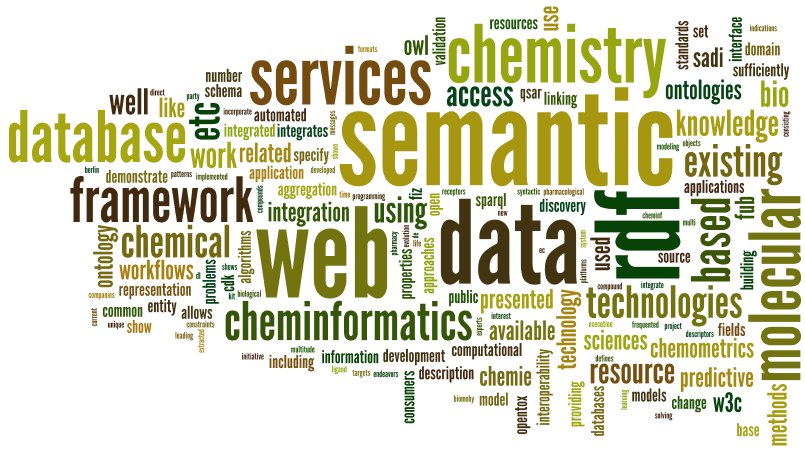
\includegraphics[width=0.5\textwidth]{graphics/wordle_cinf003} 

  \subsection*{Figure 2 - Keyword cloud for the \textit{RDF and Ontologies} session.}
  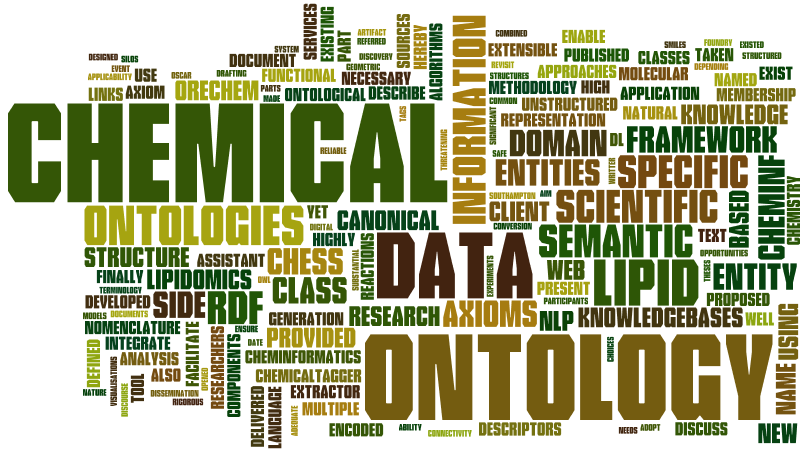
\includegraphics[width=0.5\textwidth]{graphics/wordle_cinf0031} 

  \subsection*{Figure 3 - Keyword cloud for the \textit{RDF and Chemical Applications} session.}
  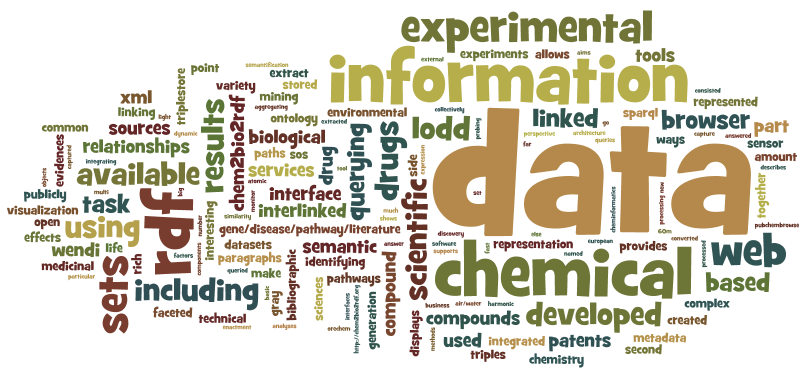
\includegraphics[width=0.5\textwidth]{graphics/wordle_cinf0032} 

  \subsection*{Figure 4 - Web page using SPARQL to visualize alkane boiling points extracted
    from another web page.}
  Web page with JavaScript by Jankowski visualizing the boiling point of a series of
  alkanes from Wiener~\cite{Wiener1947} extracted with SPARQL from a second, XHTML+RDFa web page at
  \url{http://egonw.github.com/cheminformatics.classics/classic1.html}.
  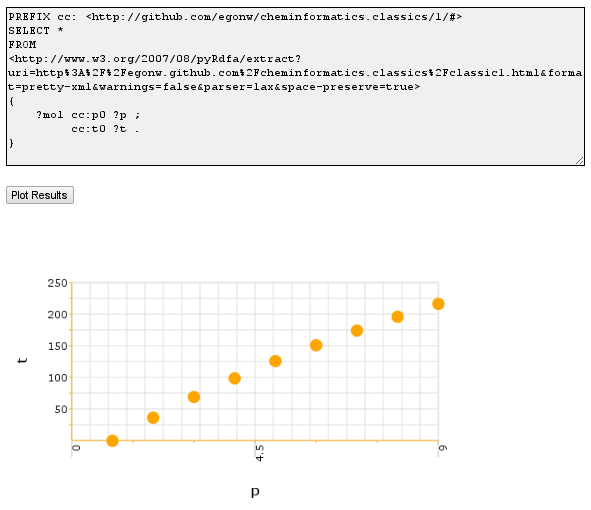
\includegraphics[width=0.7\textwidth]{graphics/sparqlGraphing1} 

\clearpage

\section*{Tables}
  \subsection*{Table 1 - Key W3C Specifications}
    Several of the key specifications and when they were
    recommended by the World Wide Web Consortium. \par \mbox{}
    \par
    \mbox{
      \begin{tabular}{lll}
        Year & Technology & Description \\ 
        \hline
        1999 & RDF     & Resource Description Framework (RDF) Model and Syntax Specification~\cite{Lassila1999} \\
        2004 & RDF/XML & RDF/XML Syntax Specification (Revised)~\cite{Beckett2004} \\
             & RDF     & Resource Description Framework (RDF): Concepts and Abstract Syntax~\cite{Carroll2004}  \\
             & OWL     & OWL Web Ontology Language Overview~\cite{OWL22009}\\
        2007 & OWL2    & OWL 2 Web Ontology Language Document Overview~\cite{OWL22009}  \\
        2008 & RDFa    & RDFa in XHTML: Syntax and Processing~\cite{RDFA2008} \\
             & SPARQL  & SPARQL Query Language for RDF~\cite{PrudHommeaux2008} \\
      \end{tabular}
      }


\end{bmcformat}
\end{document}







